\documentclass{standalone}
\usepackage{tikz}
\usetikzlibrary{calc,arrows}
\usetikzlibrary{decorations.pathreplacing,calligraphy}
\usepackage{pgfplots}
\usetikzlibrary{intersections, pgfplots.fillbetween}
\usetikzlibrary{snakes}
\usepackage{xcolor}

\begin{document}

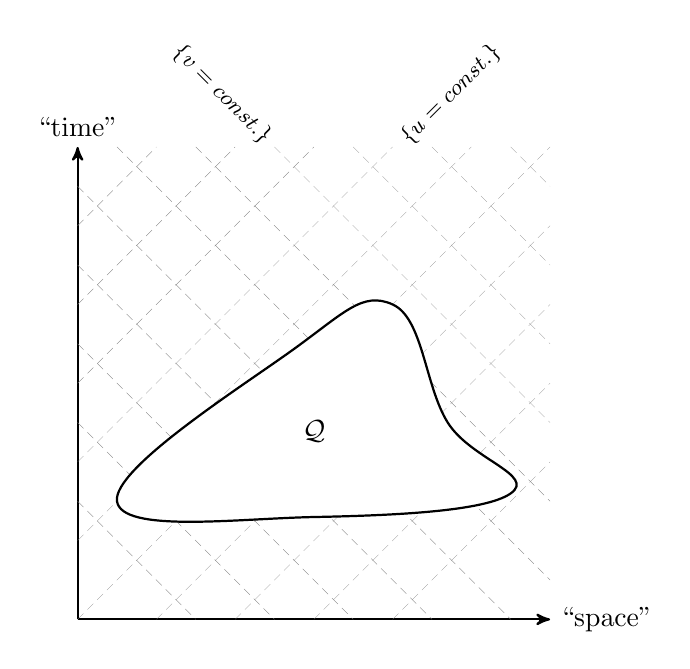
\begin{tikzpicture}[scale=1]

\coordinate (n1) at (0,0) {};

\draw[thick, ->, >=stealth'] (0,0)  -- (6,0) node(xline)[right] {``space"};
\draw[thick, ->, >=stealth'] (0,0)  -- (0,6) node(xline)[above] {``time"};


\draw[ultra thin, gray, densely dashed] (0,5) -- (1,6);
\draw[ultra thin, gray, densely dashed] (0,4) -- (2,6);
\draw[ultra thin, gray, densely dashed] (0,3) -- (3,6);
\draw[ultra thin, gray, densely dashed] (0,2) -- (4,6);
\node[label = {[rotate = 45 ,xshift = 2mm, yshift=3mm]above:\footnotesize	 $\{u =  const. \}$  }] at (5,6) {};
\draw[ultra thin, gray, densely dashed] (0,1) -- (5,6);
\draw[ultra thin, gray, densely dashed] (0,0) -- (6,6);
\draw[ultra thin, gray, densely dashed] (1,0) -- (6,5);
\draw[ultra thin, gray, densely dashed] (2,0) -- (6,4);
\draw[ultra thin, gray, densely dashed] (3,0) -- (6,3);
\draw[ultra thin, gray, densely dashed] (4,0) -- (6,2);


\draw[ultra thin, gray, densely dashed] (5.5,6) -- (6,5.5);
\draw[ultra thin, gray, densely dashed] (4.5,6) -- (6,4.5);
\draw[ultra thin, gray, densely dashed] (3.5,6) -- (6,3.5);
\draw[ultra thin, gray, densely dashed] (2.5,6) -- (6,2.5);
\draw[ultra thin, gray, densely dashed] (1.5,6) -- (6,1.5);
\draw[ultra thin, gray, densely dashed] (0.5,6) -- (6,0.5);
\draw[ultra thin, gray, densely dashed] (0,5.5) -- (5.5,0);
\draw[ultra thin, gray, densely dashed] (0,4.5) -- (4.5,0);
\draw[ultra thin, gray, densely dashed] (0,3.5) -- (3.5,0);
\draw[ultra thin, gray, densely dashed] (0,2.5) -- (2.5,0);
\draw[ultra thin, gray, densely dashed] (0,1.5) -- (1.5,0);

\node[label = {[rotate = -45 ,xshift = -5mm, yshift=0mm]above:\footnotesize	 $\{v =  const. \}$  }] at (2,6) {};

\draw[thick, fill = white] plot [smooth cycle, tension=.7] 
    coordinates {(.5,1.5)(3,1.3)(5.5,1.6)(4.7,2.5)(4,4)(2.7,3.4)};

\node[label = {$\mathcal{Q}$}] at (3,2) {};
  


\end{tikzpicture}

\end{document}